\chapter{Probability distributions closeness}
Some methods were developed to assess closeness between different probability distributions (see Figure \ref{fig:diffkl}).

In this appendix, we cover the ones which are used in the thesis.

\begin{figure}[h]
    \centering
    \subfigure{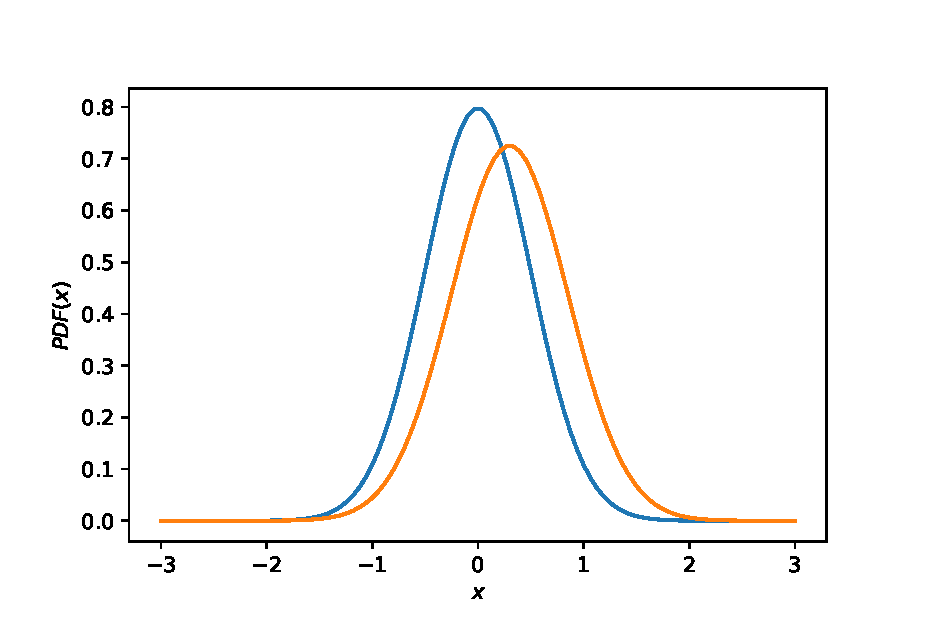
\includegraphics[width=0.5\textwidth]{images/diff-kl-1}}%
    \hfill
    \subfigure{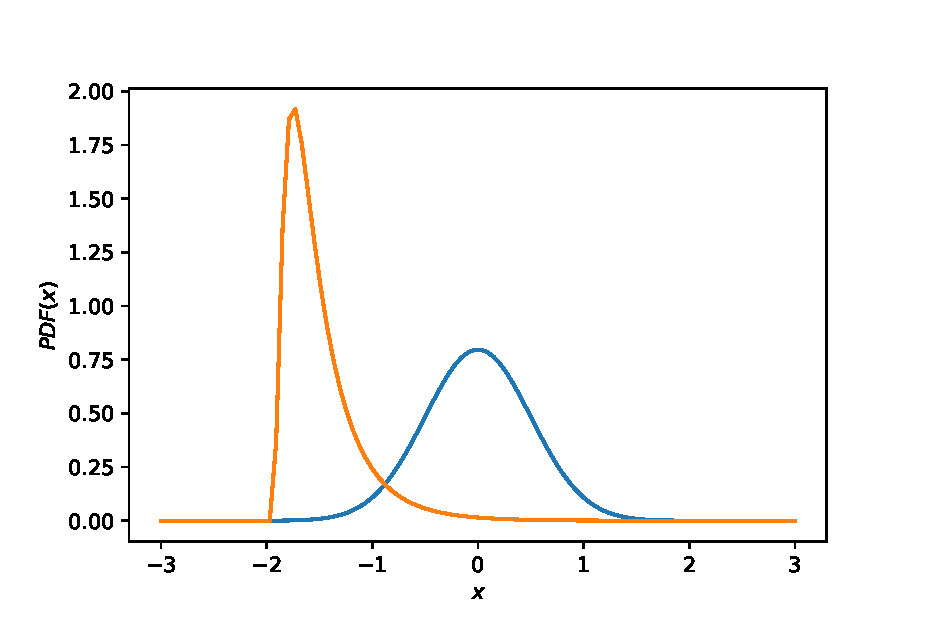
\includegraphics[width=0.5\textwidth]{images/diff-kl-2}}
    \caption{On the left plot the probability density function of two close distributions, the opposite on the right plot.}
    \label{fig:diffkl}
\end{figure}

\section{Kullback–Leibler divergence}
Given two probability distributions $p(x)$ and $q(x)$, we define the KL divergence as:
$$ \mathit{KL}(p \| q) = \int_x p(x) \log_2 \frac{p(x)}{q(x)} = \E_{X \sim p}{[\log_2 \frac{p(x)}{q(x)}]}$$

If the two distributions are discrete, it can be rewritten as:
$$ \mathit{KL}(p \| q) = \sum_i p(i) \log_2 \frac{p(i)}{q(i)}$$

Suppose we have two Categorical distributions $c_1$ and $c_2$ with parameters $p_{c_1} = (0.1, 0.2, 0.7)$ and $p_{c_2} = (0.3, 0.5, 0.2)$, respectively.

Given the formula presented above, we can compute the KL divergence:
\begin{itemize}
    \item $\mathit{KL}(c_1 \| c_2) = 0.1 \log_2 \frac{0.1}{0.3} + 0.2 \log_2 \frac{0.2}{0.5} + 0.7 \log_2 \frac{0.7}{0.2} \approx 0.85$
    \item $\mathit{KL}(c_2 \| c_1) = 0.3 \log_2 \frac{0.3}{0.1} + 0.5 \log_2 \frac{0.5}{0.2} + 0.2 \log_2 \frac{0.2}{0.7} \approx 0.77$
\end{itemize}


\subsection{Proprieties}
From the previous example, it can be seen that the KL divergence is not symmetric: $\mathit{KL}(p \| q) \neq \mathit{KL}(q \| p)$.

Also, note that $\mathit{KL}(p \| p) = \int_x p(x) \log_2 \frac{p(x)}{p(x)} = \int_x p(x) \log_2 (1) = \int_x p(x) \cdot 0 = 0$
and $\mathit{KL}(p \| q) \geq 0$.

\subsection{Considerations about symmetry}

If we want to model a probability distribution $z$ to be close to another probability distribution $p$, we have to ask ourselves if we need to minimize $\mathit{KL}(z \| p)$ or $\mathit{KL}(p \| z)$.

In the case of $\min_{z} \mathit{KL}(z \| p) = \min \int_x z(x) \log_2 \frac{z(x)}{q(x)}$, there exist a trivial solution which assigns low values to $z(x)$ when $q(x)$ is large.
This leads to a solution $z$ which is very different from $p$ but has a small KL-divergence $\mathit{KL}(z \| p)$.
Note that also $\min_{z} \mathit{KL}(z \| p)$ is not defined if $p(i)=0$ for one value of $i$ at least.
For these reasons, $\mathit{KL}(p \| z)$ is used instead of $\mathit{KL}(z \| p)$ to measure how well $z$ approximates $p$.

\section{Hellinger distance}
The Hellinger distance has some advantages over the Kullback–Leibler divergence:
\begin{itemize}
    \item it is symmetric: $\mathit{HD}(p, q) = \mathit{HD}(q, p)$
    \item it has an upper bound: $0 \leq \mathit{HD}(p, q) \leq 1$
\end{itemize}

Given two discrete probability distributions $p$ and $q$, the Hellinger distance is defined as:
$$\mathit{HD}(p, q) = \mathit{HD}(q, p) = \frac{1}{\sqrt{2}} \sqrt{\sum_i (\sqrt{p(i)} - \sqrt{q(i)})^2}$$